% !TEX root = Thesis.tex

%==============================================================================
\chapter{Diffraction of a \acl{bec} with a one-dimensional Optical lattice}
\label{chap:one_dimensional_lattices}
%==============================================================================
In ultracold atoms physics, Optical lattices are defined as periodic standing wave potentials generated by interfering laser beams. Its use allows to replicate results from solid state physics, with the interaction between an ultracold atomic ensemble and an optical lattice being equivalent to the role of electrons in an atomic lattice \cite{Lewenstein2007, Bloch2008}.  However, the use of ultracold systems presents some advantages when comparing with those used in solid state physics. The main one being the capability of changing the optical lattice properties, by simply adjusting the intensity and detuning of the laser beams forming it. An additional advantage of ultracold atomic systems is the non-existence of crystal defects, which can be a big source of noise in solid states systems \cite{VanDerZiel1978}. This experiment will seek to study how an erbium \ac{bec} behaves when interacting with a one-dimensional optical lattice. In this chapter, an introduction describing the theory behind optical lattices will be shown. After this, it follows a brief description of the implemented set up to form the lattice by using the \SI{841}{\nano\meter} erbium transition (see Table \ref{tab:Transitions}).

\section{Theoretical description of an Optical lattice}

As previously mentioned, generating an optical lattice requires the use of two interfering laser beams. Taken individually, each would interact with the atomic cloud like a typical \acf{odt}. Therefore, each beam generates a dipole potential in the atomic ensemble given by Equation \eqref{eq:interaction_potential}. However, in this case there is not a far detuning between the laser beams forming the lattice and erbium atomic transitions. Due to this, assuming the optical fields as quasi-electrostatic does not work any more. But, Equation \eqref{eq:interaction_potential} holds in any case and can be rewritten when the atoms are approximated as a two level scheme following the behaviour of a classical Lorentz oscillator \cite{Grimm2000}. For this case, it can be proved that the complex polarizability $\alpha$ has the form:

\begin{equation}\label{eq:complex_polarizability}
	\alpha = 6 \pi \epsilon_0 c^3 \frac{\Gamma/\omega_0^2}{\omega_0^2 -\omega^2 -i(\omega^3/\omega_0^2)\Gamma} 
\end{equation} 

Where $\omega$ is the optical frequency of the laser beam interacting with the atom ensemble, $\omega_0$ is the atomic transition and $\Gamma$ the on-resonance damping rate. For the classical Lorentz oscillator, this rate is equivalent to $\Gamma = \Gamma_\text{cls}$ where:
\begin{equation}\label{eq:classical_damping_rate}
	\Gamma_\text{cls} = \frac{e^2 \omega_0^2}{6\pi\epsilon_0m_ec^3}
\end{equation}

With $e$ and $m_e$ representing the electron charge and mass respectively. Even though this result is obtained when using the classical Lorentz approximation, an equivalent result can be obtained when considering the semi-classical model of the atom. In which, the atom is considered as a two-level quantum system that interacts with a classical field of light. For the semi-classical model, Equation \eqref{eq:complex_polarizability} is still valid, except for the damping rate $\Gamma$. Now, it corresponds to the spontaneous decay rate of the excited level $\Gamma_\text{smcls} \equiv \gamma$ and is given by

\begin{equation}\label{eq:semiclassical_damping_rate}
	\Gamma_\text{smcls} = \frac{\omega_0^3}{3\pi\epsilon_0 \hbar c^3} \mathopen|\bra{e}\mu\ket{g}\mathclose|^2
\end{equation}

Where $\bra{e}\mu\ket{g}$ stands for the dipole matrix element between ground and excited state. By using Equations \eqref{eq:interaction_potential} and \eqref{eq:complex_polarizability}, for the case of large enough detuning $\delta$ ( making the scattering rate much smaller than $\Gamma$) and low enough intensities $I(\vec{r})$ (avoiding saturation of the excited state), the dipole potential $U_{\text{dip}}(\vec{r})$ can be obtained as

\begin{equation}
	U_{\text{dip}}(\vec{r}) = -\frac{3\pi c^2}{2\omega_0^3} \bigg(\frac{\Gamma}{\omega_0-\omega} + \frac{\Gamma}{\omega_0+\omega}\bigg) \cdot I(\vec{r})
\end{equation} 

Being this equation valid for both the classical and semi-classical model. For most cases, the rotating wave approximation can be applied here because usually $\mathopen|\delta\mathclose| << \omega_0$. Using this approximation, the dipole potential for one laser beam interacting with an neutral atomic ensemble can be obtained as

\begin{equation}\label{eq:relation_potential_intensity}
	U_{\text{dip}}(\vec{r}) = \frac{3\pi c^2 \Gamma}{2\omega_0^3 \delta} \cdot I(\vec{r})
\end{equation} 

And by assuming the beam to be a Gaussian beam, Equations \eqref{eq:intensity_gaussian} and \eqref{eq:relation_potential_intensity} lead to the exponential behaviour already described in Equation \eqref{eq:dipole_potential}. 

\begin{figure}[!htbp]\centering
	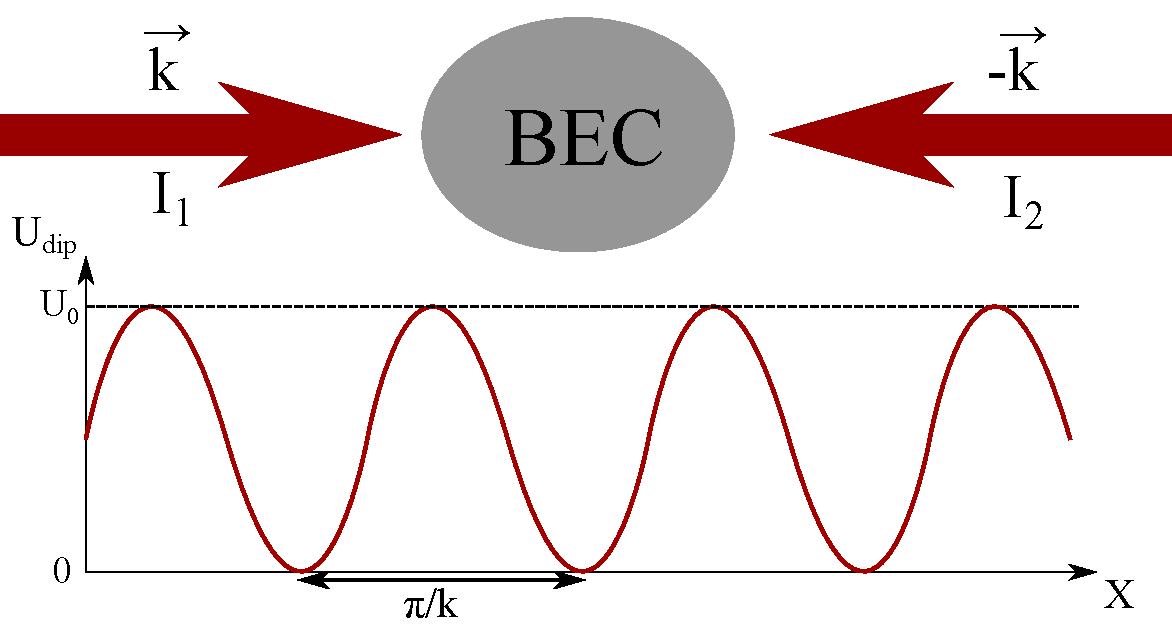
\includegraphics[width=1.\columnwidth]{lattice_beams.pdf}
	\caption[]{}\label{fig:lattice_beams}
\end{figure}

After considering only the interaction with just one beam, the optical potential $U_\text{lat}(\vec{r})$ for the lattice forming two counter propagating beams has the same relation with the lattice intensity $I_\text{lat}(\vec{r})$ than the previous case:

\begin{equation}\label{eq:relation_lattice_potential_intensity}
	U_{\text{lat}}(\vec{r}) = \frac{3\pi c^2 \Gamma}{2\omega_0^3 \delta} \cdot I_{\text{lat}}(\vec{r})
\end{equation} 

Where $I_\text{lat}(\vec{r})$ can be 

\iffalse
It must be noted that this semi-classical model uses the electric dipole approximation, which assumes the laser transition to have a wavelength way greater that the typical size of the atom. This is a reasonable approximation for most of the cases but will be considered as a possible source of errors in our model.
\fi

%%% Local Variables: 
%%% mode: latex
%%% TeX-master: "Thesis"
%%% End: 
